% !TeX root = ../hw4.tex
\section{Reproducing the Gray-Scott Patterns}

\subsection{Statement}
Reproduce the Gray-Scott patterns $\alpha$, $\lambda$, $\mu$, and $\theta$ shown in \autoref{prob5:fig:patterns}.

\begin{figure}[H]
    \centering
    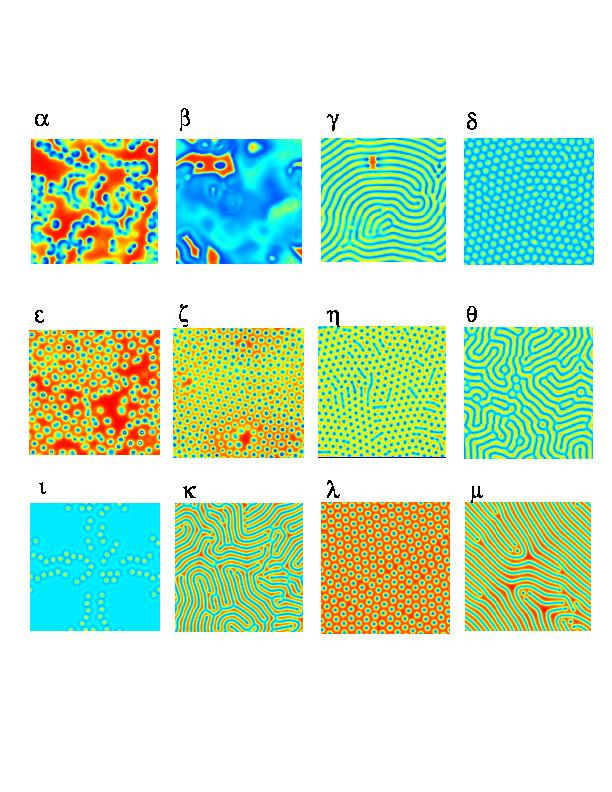
\includegraphics[width=0.6\textwidth]{figures/reactions/patterns.jpg}
    \caption{The labeled Gray-Scott patterns}\label{prob5:fig:patterns}
\end{figure}

\subsection{Method}

The Gray-Scott Model models reaction diffusion of two chemicals $U$ and $V$ in an unstirred planar chemical reactor.
Further, we assume the reaction $U \to V$ is autocatalyzed by the presence of $V$.
More specifically, the Gray-Scott model assumes the cubic autocatalysis
\begin{equation}
    U + 2V \to 3V
\end{equation}
with reaction rate $kuv^2$.
This reaction can be modeled according to the following system of differential equations.\footnote{I'm smashing my giant red ``I Believe'' button on this one. My chemistry is a little rusty, and PDEs give me heart palpitations.}
\begin{equation}
    \begin{cases}
        \displaystyle{\frac{\partial u}{\partial t} = r_u \Delta u - uv^2 + f(1 - u)} \\[10pt]
        \displaystyle{\frac{\partial v}{\partial t} = r_v \Delta v + uv^2 - (f + k)v}
    \end{cases}\label{prob5:eqn:gray-scott}
\end{equation}
where $u$ and $v$ are the concentrations, and $r_u$ and $r_v$ are the diffusion rates, of $U$ and $V$ respectively.
The chemical $U$ is added to the reactor at the feed rate $f$ which is scaled by the concentration of $U$.
Simultaneously, $U$ and $V$ are drained from the reactor at the kill rate $k$, which is scaled by $f$ and the concentration of $V$.

Recall that the Laplacian operator $\displaystyle\Delta f(x, y, t) = \nabla^2 f(x, y, t) = \frac{\partial^2 f}{\partial x^2} + \frac{\partial^2 f}{\partial y^2}$ can be discretized as
\begin{align}
    \Delta f(x, y, t) \approx \frac{f(x - h, y, t) + f(x + h, y, t) + f(x, y - h, t) + f(x, y + h, t) - 4f(x, y)}{h^2}\label{prob5:eqn:discrete-laplacian-operator}
\end{align}
for fixed step size $h$, uniform in both spatial dimensions --- allowing us to collect more of the terms together.
In this problem, we have $\Delta x = \Delta y = \Delta t = h = 1$.

However, note that the numerical computation of $\Delta f$ over a large spatial domain is computationally intensive, despite being relatively simple.
Therefore, we desire a a method where the Laplacian can be applied to $f$ over each element of the spatial domain at once.

Let $\mathbf U$ be a square $n \times n$ matrix of concentrations.
We then unravel $\mathbf U$ into a column vector $\vec u$ and left-multiply by an $n^2 \times n^2$ matrix $\mathbf L$ to numerically compute the discrete Laplacian over the entire spatial domain.

That is, the discretized version of \autoref{prob5:eqn:gray-scott} becomes
\begin{eqnarray}
    \begin{cases}
        \vec u_{t + 1} & = \vec u_t + r_u \mathbf L \cdot \vec u_t - \vec u_t \cdot \vec {v_t}^2 + f(1 - \vec u_t) \\
        \vec v_{t + 1} & = \vec v_t + r_v \mathbf L \cdot \vec v_t + \vec u_t \cdot \vec {v_t}^2 - (f + k)\vec v_t
    \end{cases}\label{prob5:eqn:discretized-gray-scott}
\end{eqnarray}
where the vector product $\vec u_t \cdot \vec {v_t}^2$ is computed component-wise.

Then the $n ^2 \times n^2$ matrix $\mathbf L$ is the block diagonal matrix
\begin{equation}
    \mathbf L = \begin{bmatrix}
        L_n    & I_n    & 0_n    & \cdots & 0_n    & I_n    \\
        I_n    & L_n    & I_n    & 0_n    & \cdots & 0_n    \\
        0_n    & I_n    & L_n    & I_n    & \ddots & \vdots \\
        \vdots & \ddots & \ddots & \ddots & \ddots & 0_n    \\
        0_n    & \cdots & 0_n    & I_n    & L_n    & I_n    \\
        I_n    & 0_n    & \cdots & 0_n    & I_n    & L_n
    \end{bmatrix}\label{prob5:eqn:laplacian}
\end{equation}
where the $0_n$ blocks are the $n \times n$ zero matrix, and the $I_n$ blocks are the $n \times n$ identity matrix.
The $L_n$ blocks are the $n \times n$ diagonal matrix
\begin{equation}
    L_n = \begin{bmatrix}
        -4     & 1      & 0      & \cdots & 0      & 1      \\
        1      & -4     & 1      & 0      & \cdots & 0      \\
        0      & 1      & -4     & 1      & \ddots & \vdots \\
        \vdots & \ddots & \ddots & \ddots & \ddots & 0      \\
        0      & \cdots & 0      & 1      & -4     & 1      \\
        1      & 0      & \cdots & 0      & 1      & -4
    \end{bmatrix}\label{prob5:eqn:laplacian-L-block}
\end{equation}

Now, $\mathbf L$ is appropriate for periodic boundary conditions.
If homogeneous Dirichlet boundary conditions are desired, we use the matrix
\begin{equation}
    \mathbf L_d = \begin{bmatrix}
        L_n              & I_n    & 0_n    & \cdots & 0_n    & \color{red}{0_n} \\
        I_n              & L_n    & I_n    & 0_n    & \cdots & 0_n              \\
        0_n              & I_n    & L_n    & I_n    & \ddots & \vdots           \\
        \vdots           & \ddots & \ddots & \ddots & \ddots & 0_n              \\
        0_n              & \cdots & 0_n    & I_n    & L_n    & I_n              \\
        \color{red}{0_n} & 0_n    & \cdots & 0_n    & I_n    & L_n
    \end{bmatrix}
\end{equation}
and the modified $L_n$ block
\begin{equation}
    L_n = \begin{bmatrix}
        -4             & 1      & 0      & \cdots & 0      & \color{red}{0} \\
        1              & -4     & 1      & 0      & \cdots & 0              \\
        0              & 1      & -4     & 1      & \ddots & \vdots         \\
        \vdots         & \ddots & \ddots & \ddots & \ddots & 0              \\
        0              & \cdots & 0      & 1      & -4     & 1              \\
        \color{red}{0} & 0      & \cdots & 0      & 1      & -4
    \end{bmatrix}
\end{equation}
If homogeneous Neumann boundary conditions are desired, further modifications must be made to the main diagonal of $\mathbf L_d$ to maintain 0-sum rows.\footnote{
    Online material on the discretized Laplacian is lacking in general, and much more so related to periodic boundary conditions.
    I found exactly one source that discussed the discretized Laplacian with periodic boundary conditions in more than one sentence.

    A PDF of \textit{Computational Methods for Inverse Problems} may be found on \href{http://booksdescr.org/item/index.php?md5=6DF2AA596DDBE34BCF9354A5626B75DA}{Library Genesis}.
    The relevant pages are 74--75.
}

\subsection{Implementation}
The discrete Laplacian in \autoref{prob5:eqn:laplacian} can be generated with
\begin{minted}{python}
    def laplacian(N):
        """Compute a matrix that performs the discretized Laplacian in 2D."""
        e = np.ones(N ** 2, dtype=int)
        return sp.sparse.spdiags(
            data=[-4 * e, e, e, e, e, e, e],
            diags=[0, -1, 1, -N, N, -(N ** 2 - N), N ** 2 - N],
            m=N ** 2,
            n=N ** 2,
        )
\end{minted}
Notice that we use a sparse representation for $\mathbf L$.
The images we generated are $256 \times 256$, which would produce a $65536 \times 65536$ matrix $\mathbf L$ of 64-bit doubles, which would take roughly 32GB of memory to store.
Thus it is quite important to use a sparse representation, along with the corresponding sparse matrix multiplication algorithms.

Note that our implementation does \textit{not} include the 1's in the outer corners of the $L_n$ blocks of $\mathbf L$.
Every source we've looked at includes them, but when used, we are quickly overwhelmed by numerical overflow in only a few iterations.
Removing the outer 1's while leaving the outer $I_n$ blocks still implements periodic boundary conditions everywhere except the four corners of the domain.

This behavior can be observed by working out the matrix multiplications ``by-hand''\footnote{With Python, that is.} with various initial configurations of the domain.
What we observed was one iteration of applying the $\mathbf L$ matrix as stated had the intended diffusion effect that correctly wrapped around the domain boundaries --- but only as long as the domain was all zeros, with a few hot-spots of high concentrations.
The diffusion did not work properly, even in the first iteration, with an all ones domain, with a few hot-spots.
What we observed in the second case was that the left and right edge of the domain would accumulate high concentrations, while the rest of the domain would diffuse as expected.

In the first few iterations, that is.
As mentioned, we were quickly overwhelmed with numerical error, causing a flood of NaNs within 100 iterations.

If the outer $I_n$ blocks of $\mathbf L$ were left alone, and the outer 1's of the $L_n$ blocks we removed, the diffusion worked as intended, except at the corner cells.
While this is concerning from a numerical methods standpoint, we are prepared to smash our ``I Believe'' buttons\footnote{Side note: I have not been able to find any ``I Believe'' buttons for sale online, so I believe\texttrademark{} there is strong a business opportunity in the SD Mines Mathematics department.} and pretend there is no issue here.

Online sources are not even consistent with their formulation of the $\mathbf L$ matrix.
Some use 2's along the diagonal instead of 4's, others vary the formulation of the two $I_n$ diagonals around the main diagonal, and still others vary the formulation of the top left and bottom right corners.

So we picked what behaved well experimentally, and did not look back.

The initial concentrations of $U$ and $V$ can be generated by
\begin{minted}{python}
    def init(N, scale, r, u0, v0):
        """Initialize the U, V concentrations."""
        u, v = np.ones((N, N)), np.zeros((N, N))
        u += scale * np.random.random((N, N))
        v += scale * np.random.random((N, N))
        c = N // 2
        if r is not None:
            u[c - r : c + r, c - r : c + r] = u0
            v[c - r : c + r, c - r : c + r] = v0
        return u, v
\end{minted}
Notice that we enabled several tweakable parameters to explore the impact the random initial concentrations of $U$ and $V$ have on the created patterns.
There are two methods of random initialization that can be combined at will:
\begin{enumerate}
    \item Random values distributed uniformly throughout the spatial domain
    \item A high concentration square in the center of the domain
\end{enumerate}

Then \autoref{prob5:eqn:discretized-gray-scott} system of equations can be applied for a given number of unit time steps with
\begin{minted}{python}
    def gray_scott(N, iters, ru, rv, f, k, scale, r, u0, v0):
    """Run the Gray-Scott model with the given parameters."""
    u, v = init(N, scale=scale, r=r, u0=u0, v0=v0)
    L = laplacian(N)
    u = u.reshape(N * N)
    v = v.reshape(N * N)

    for _ in range(iters):
        uvv = u * v ** 2
        u += ru * L.dot(u) - uvv + f * (1 - u)
        v += rv * L.dot(v) + uvv - (f + k) * v

    return u.reshape((N, N)), v.reshape((N, N))
\end{minted}

We then wrote a simple Python script to run the model with any number of tweakable parameters.
The script's commandline usage is given below
\begin{minted}{text}
    usage: reaction.py [-h] [--gui] [--output OUTPUT] [--title TITLE] [--uv]
                    [--size SIZE] [--ru RU] [--rv RV] [--feed FEED]
                    [--kill KILL] [--iterations ITERATIONS] [--radius RADIUS]
                    [--u0 U0] [--v0 V0] [--scale SCALE]

    Run the Gray-Scott Model with configurable parameters.

    optional arguments:
    -h, --help            show this help message and exit

    --gui                 Open a GUI window displaying the plot.
    --output OUTPUT, -o OUTPUT
                          The filename to save the results as.
    --title TITLE         The plot title.
    --uv                  Plot both U and V concentrations.

    --size SIZE, -n SIZE  The grid size.
    --ru RU               The U diffusion rate.
    --rv RV               The V diffusion rate.
    --feed FEED, -f FEED  The U feed rate.
    --kill KILL, -k KILL  The U,V kill rate.
    --iterations ITERATIONS, -i ITERATIONS
                          The number of iterations.

    --radius RADIUS, -r RADIUS
                          The initial high concentration center radius.
    --u0 U0               The initial high concentration center U concentration.
    --v0 V0               The initial high concentration center V concentration.
    --scale SCALE, -s SCALE
                          The scale of the initial uniform distribution.
\end{minted}

\subsection{Results}
The $f$ and $k$ parameters largely decide the pattern displayed at the end of a large number of iterations.
The mappings for the patterns shown in \autoref{prob5:fig:patterns} are shown in \autoref{prob5:fig:pattern-mappings}.
\begin{figure}[H]
    \centering
    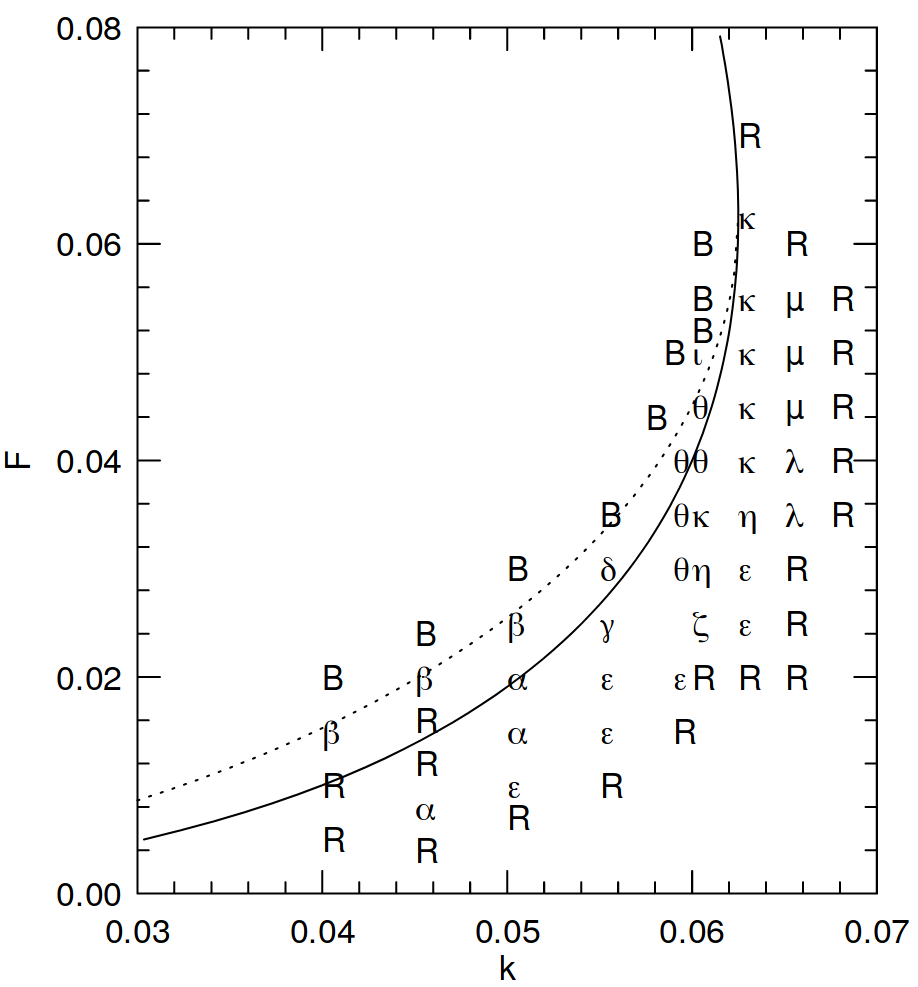
\includegraphics[width=0.6\textwidth]{figures/reactions/pattern-mappings.png}
    \caption{The parameter mappings to the patterns shown in \autoref{prob5:fig:patterns}}\label{prob5:fig:pattern-mappings}
\end{figure}

Our results are shown in \autoref{prob5:fig:results}.
For ease of pattern comparisons, \autoref{prob5:fig:patterns} is duplicated below.

\begin{figure}[H]
    \centering
    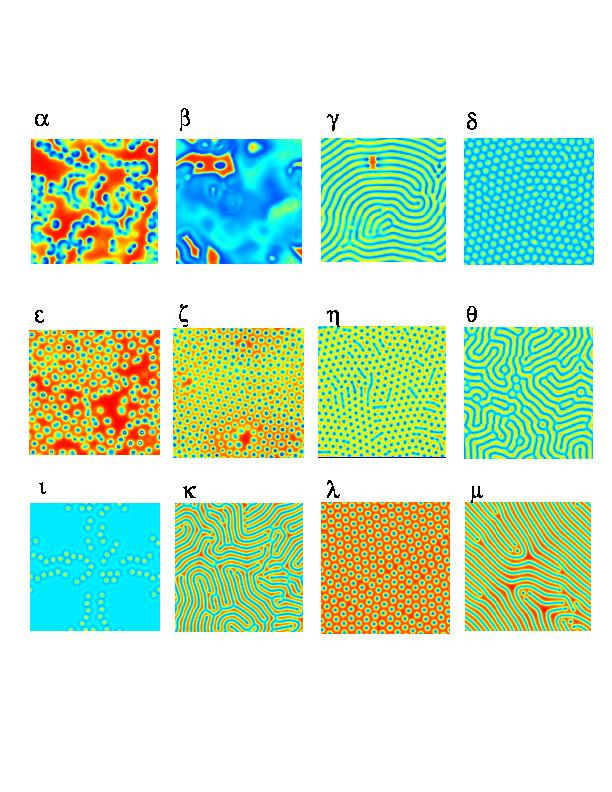
\includegraphics[width=0.6\textwidth]{figures/reactions/patterns.jpg}
    \caption{The labeled Gray-Scott patterns}
\end{figure}

% NOTE: These images will be created by the makefile if they are not present.
% However, they take *quite* some time to generate, so it's advisable to set
% $(REACTION_SIZE) and $(REACTION_ITERS) to small values in the Makefile first.
\begin{figure}[H]
    \captionsetup[subfigure]{labelformat=empty}
    \centering
    \begin{subfigure}[t]{0.25\textwidth}
        \centering
        \includegraphics[width=\textwidth]{figures/reactions/alpha.eps}
        \caption{$(\alpha)$}
    \end{subfigure}%
    \begin{subfigure}[t]{0.25\textwidth}
        \centering
        \includegraphics[width=\textwidth]{figures/reactions/beta.eps}
        \caption{$(\beta)$}
    \end{subfigure}%
    \begin{subfigure}[t]{0.25\textwidth}
        \centering
        \includegraphics[width=\textwidth]{figures/reactions/gamma.eps}
        \caption{$(\gamma)$}
    \end{subfigure}%
    \begin{subfigure}[t]{0.25\textwidth}
        \centering
        \includegraphics[width=\textwidth]{figures/reactions/delta.eps}
        \caption{$(\delta)$}
    \end{subfigure}%

    \begin{subfigure}[t]{0.25\textwidth}
        \centering
        \includegraphics[width=\textwidth]{figures/reactions/epsilon.eps}
        \caption{$(\varepsilon)$}
    \end{subfigure}%
    \begin{subfigure}[t]{0.25\textwidth}
        \centering
        \includegraphics[width=\textwidth]{figures/reactions/zeta.eps}
        \caption{$(\zeta)$}
    \end{subfigure}%
    \begin{subfigure}[t]{0.25\textwidth}
        \centering
        \includegraphics[width=\textwidth]{figures/reactions/eta.eps}
        \caption{$(\eta)$}
    \end{subfigure}%
    \begin{subfigure}[t]{0.25\textwidth}
        \centering
        \includegraphics[width=\textwidth]{figures/reactions/theta.eps}
        \caption{$(\theta)$}
    \end{subfigure}%

    \begin{subfigure}[t]{0.25\textwidth}
        \centering
        \includegraphics[width=\textwidth]{figures/reactions/iota.eps}
        \caption{$(\iota)$}
    \end{subfigure}%
    \begin{subfigure}[t]{0.25\textwidth}
        \centering
        \includegraphics[width=\textwidth]{figures/reactions/kappa.eps}
        \caption{$(\kappa)$}
    \end{subfigure}%
    \begin{subfigure}[t]{0.25\textwidth}
        \centering
        \includegraphics[width=\textwidth]{figures/reactions/lambda.eps}
        \caption{$(\lambda)$}
    \end{subfigure}%
    \begin{subfigure}[t]{0.25\textwidth}
        \centering
        \includegraphics[width=\textwidth]{figures/reactions/mu.eps}
        \caption{$(\mu)$}
    \end{subfigure}%
    \caption{Reproductions of the Gray-Scott patterns}\label{prob5:fig:results}
\end{figure}

Notice that we were even able to reproduce the color scheme --- as scarring as doing so was.\footnote{
    The ``Jet'' colormap should \textit{not} be used.
    Full stop.
    It creates contrast where there is none; a slight perturbation of your data might push a small dimly-colored region of your plot into a bright attention-grabbing ``feature''.
    That is, ``Jet'' produces features in your data that is not there.
    In technical terms, ``Jet'' is not perceptually uniform; values in the range $[0.1, 0.3]$ will not produce colors with the same visual range as values in the range $[0.6, 0.8]$.

    There are a great number of online resources demonstrating the inferiority of the ``Jet'' colormap:
    \begin{itemize}
        \item \url{https://jakevdp.github.io/blog/2014/10/16/how-bad-is-your-colormap/}
        \item \url{https://bids.github.io/colormap/}
        \item \url{http://medvis.org/2016/02/23/better-than-the-rainbow-the-matplotlib-alternative-colormaps/}
        \item \url{http://medvis.org/2012/08/21/rainbow-colormaps-what-are-they-good-for-absolutely-nothing/}
    \end{itemize}
}

The values used to generate the patterns in \autoref{prob5:fig:results} are summarized in \autoref{prob5:tab:parameters}.
The parameter $r$ is the radius of the initial center concentration of the $U$ and $V$ chemicals.
The $s$ parameter is the scale of the random values uniformly added throughout the reactor.

\begin{table}[H]
    \centering
    \caption{The parameters used to reproduce the Gray-Scott patterns}\label{prob5:tab:parameters}
    \begin{tabular}{@{}lllllll@{}}
        \toprule
        pattern       & $k$    & $f$   & $r$ & $s$  & iterations & time (mm:ss) \\ \midrule
        $\alpha$      & 0.05   & 0.017 & 5   & 0.02 & 10000      & 2:03         \\
        $\beta$       & 0.045  & 0.019 & 2   & 0.02 & 10000      & 2:03         \\
        $\gamma$      & 0.052  & 0.021 & 5   & 0.02 & 20000      & 0:48         \\
        $\delta$      & 0.052  & 0.026 & 5   & 0.02 & 10000      & 2:02         \\
        $\varepsilon$ & 0.052  & 0.017 & 2   & 0.02 & 10000      & 2:04         \\
        $\zeta$       & 0.06   & 0.023 & 2   & 0.1  & 10000      & 2:03         \\
        $\eta$        & 0.06   & 0.028 & 2   & 0.1  & 10000      & 2:03         \\
        $\theta$      & 0.06   & 0.04  & 2   & 0.1  & 10000      & 0:58         \\
        $\iota$       & 0.06   & 0.054 & 2   & 0.2  & 10000      & 1:02         \\
        $\kappa$      & 0.064  & 0.05  & 5   & 0.2  & 10000      & 0:57         \\
        $\lambda$     & 0.066  & 0.04  & 5   & 0.02 & 20000      & 1:22         \\
        $\mu$         & 0.0665 & 0.055 & 32  & 0.1  & 20000      & 2:38         \\ \bottomrule
    \end{tabular}
\end{table}

Increasing the random scale seemed to have the effect of removing the regularity and symmetry in the generated patterns.
However, if the scale was increased too high, the reaction would cross the tipping point and converge to a uniform concentration of the two chemicals.
Increasing the radius of the initial high concentration area made the patterns spread faster --- requiring fewer iterations to display the desired patterns.
Observe also that the $\lambda$ and $\mu$ patterns required more time to develop their desired structure than the rest of the patterns.

Notice that the timings vary wildly for each of the different patterns.
This is a consequence of running the jobs in parallel and starving them for resources.
Of note, pattern $\gamma$ took 48 second to run 20,000 iterations, even though pattern $\alpha$ took a little over two minutes to run 10,000 iterations.
These differences are a result of the project makefile kicking up too many jobs in parallel on an already fairly laden system.\footnote{And by laden I mean Spotify, Discord, and Firefox were running in the background\dots}

These results were ran on the following system.

\begin{listing}[h]
    \begin{minted}{text}
    $ screenfetch
                              ./+o+-       nots@abyss
                      yyyyy- -yyyyyy+      OS: Ubuntu 18.10 cosmic
                   ://+//////-yyyyyyo      Kernel: x86_64 Linux 4.18.0-17-generic
               .++ .:/++++++/-.+sss/`      Uptime: 10d 6h 42m
             .:++o:  /++++++++/:--:/-      Packages: 2517
            o:+o+:++.`..```.-/oo+++++/     Shell: bash 4.4.19
           .:+o:+o/.          `+sssoo+/    Resolution: 7680x2160
      .++/+:+oo+o:`             /sssooo.   DE: GNOME
     /+++//+:`oo+o               /::--:.   WM: GNOME Shell
     \+/+o+++`o++o               ++////.   WM Theme: Adwaita
      .++.o+++oo+:`             /dddhhh.   GTK Theme: Yaru [GTK2/3]
           .+.o+oo:.          `oddhhhh+    Icon Theme: Numix-Circle
            \+.++o+o``-````.:ohdhhhhh+     Font: Ubuntu 12
             `:o+++ `ohhhhhhhhyo++os:      CPU: Intel Core i7-6700K @ 8x 4.4GHz
               .o:`.syhhhhhhh/.oo++o`      GPU: GeForce GTX 1080
                   /osyyyyyyo++ooo+++/     RAM: 6536MiB / 15998MiB
                       ````` +oo+++o\:
                              `oo++.
    \end{minted}
\end{listing}
